142. \begin{figure}[ht!]
\center{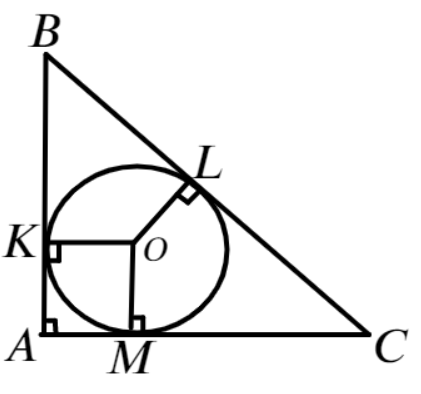
\includegraphics[scale=0.35]{g8-71.png}}
\end{figure}\\
Проведём радиусы к точкам касания. Так как отрезки касательных, проведённых из одной точки, равны, имеем $AK=AM,\ BK=BL,\ CL=CM.$ Так как $AKOM$ прямоугольник и $AK=AM,$ он является квадратом и радиус окружности тоже равен $AK.$ Пусть $AK=AM=x,$ тогда $AB=x+6,\ AC=x+4,\ BC=6+4=10$ и по теореме Пифагора для треугольника $ABC$ получаем $(x+6)^2+(x+4)^2=10^2,\ x^2+12x+36+x^2+8x+16=100,\ 2x^2+20x-48=0,\ x=2.$\\
